% ============================================================
% 2  The lattice model and its ferromagnetic transition
% ============================================================
\begin{frame}[t]
\ft{Electrons on a chain}\par
\vspace{0.6cm}
\centering
% one long chain; each term of H shown where it acts, tinted in its colour
\begin{tikzpicture}[font=\footnotesize,every pic/.style={scale=1.25}]
 % chain, fading out at both ends (sites 0..9, 1 cm apart)
 \draw[gray,thick] (-0.3,0)--(9.3,0);
 \draw[gray,thick,densely dotted] (-0.9,0)--(-0.3,0) (9.3,0)--(9.9,0);
 \foreach \i in {0,...,9} \fill[gray] (\i,0) circle (0.055);
 % hopping t: site 0 -> 1
 \onslide<1->{%
 \fill[cT!15,rounded corners=5pt] (-0.5,-0.4) rectangle (1.5,1.55);
 \pic at (0,0.42) {eup}; \pic at (1,0.42) {eghost};
 \draw[-{Stealth[length=6pt]},line width=1.3pt,cT] (0.15,0.95) to[bend left=50] (0.85,0.95);
 \node[cT,font=\small] at (0.5,1.38) {$t$};
 \node[cT] at (0.5,-0.68) {hopping};}
 % on-site U: site 3
 \onslide<2->{%
 \fill[cU!15,rounded corners=5pt] (2.45,-0.4) rectangle (3.55,1.55);
 \pic at (2.76,0.42) {eup}; \pic at (3.24,0.42) {edn};
 \node[cU,font=\small] at (3,1.2) {$U$};
 \node[cU] at (3,-0.68) {on-site};}
 % same-spin neighbours V++: sites 5,6
 \onslide<3->{%
 \fill[cVpp!15,rounded corners=5pt] (4.5,-0.4) rectangle (6.5,1.55);
 \pic at (5,0.42) {eup}; \pic at (6,0.42) {eup};
 \draw[repel,cVpp] (5.3,0.42)--(5.7,0.42);
 \node[cVpp,font=\small] at (5.5,1.2) {$V_{++}$};
 \node[cVpp] at (5.5,-0.68) {same spin};}
 % opposite-spin neighbours V+-: sites 8,9
 \onslide<4->{%
 \fill[cVpm!15,rounded corners=5pt] (7.5,-0.4) rectangle (9.5,1.55);
 \pic at (8,0.42) {eup}; \pic at (9,0.42) {edn};
 \draw[repel,cVpm] (8.3,0.42)--(8.7,0.42);
 \node[cVpm,font=\small] at (8.5,1.2) {$V_{+-}$};
 \node[cVpm] at (8.5,-0.68) {opposite spin};}
\end{tikzpicture}\par
\vspace{0.6cm}
{\small$H=$\
\colorbox{cT!15}{$\mystrut -{\color{cT}t}\sum_{i\sigma}\big(c^\dagger_{i\sigma}c^{\phantom\dagger}_{i+1,\sigma}+\text{h.c.}\big)$}
\onslide<2->{$+$\,\colorbox{cU!15}{$\mystrut{\color{cU}U}\sum_i n_{i\uparrow}n_{i\downarrow}$}}\\[5pt]
\onslide<3->{$+$\,\colorbox{cVpp!15}{$\mystrut{\color{cVpp}V_{++}}\sum_{i\sigma}n_{i\sigma}n_{i+1,\sigma}$}}
\onslide<4->{$+$\,\colorbox{cVpm!15}{$\mystrut{\color{cVpm}V_{+-}}\sum_{i\sigma}n_{i\sigma}n_{i+1,\bar\sigma}$}}\par}
\vspace{0.5cm}
\onslide<5->{%
{\small fixed filling: \colorbox{spinach!20}{\mystrut $\tfrac14$ per spin species} (a generic choice)\par}
\vspace{0.15cm}
{\small knob: \colorbox{cVpm!15}{\mystrut $\Delta V={\color{cVpm}V_{+-}}-{\color{cVpp}V_{++}}$}:\ \ opposite spins repel more\par}}
\end{frame}
% Notes: Our system: spin-1/2 electrons on a long chain. Four terms, each shown where it acts, same colour in H.
% Notes: Step 1 (green): hopping t: an electron moves to the neighbouring site. This gives a band.
% Notes: Step 2 (orange): U: two electrons (necessarily opposite spins) on the same site repel.
% Notes: Step 3 (citron): V++: same-spin electrons on neighbouring sites repel.
% Notes: Step 4 (orchid): V+-: opposite-spin electrons on neighbouring sites repel.
% Notes: Step 5: we fix the number of electrons: a quarter filling per spin (nothing special about 1/4, any generic filling would do). V++ is fixed; the knob is Delta V = V+- - V++: how much more opposite spins repel than equal spins. When opposite spins repel strongly, aligning the spins pays off: that is where the ferromagnet comes from.
\begin{frame}[t]
\ft{What each term does to magnetization}\par
\vspace{1.1cm}
\centering
% two copies of the chain: top <S^z>=0, bottom magnetized (same electron number); one term per step, marked on both
\begin{tikzpicture}[font=\footnotesize,every pic/.style={scale=1.15}]
 \def\yt{4.7}\def\yb{2.8}
 \foreach \yc in {\yt,\yb} {
   \draw[gray,thick] (-0.35,\yc)--(7.1,\yc);
   \foreach \i in {0,...,9} \fill[gray] ({0.75*\i},\yc) circle (0.055);}
 \node[anchor=east] at (-0.5,{\yt+0.42}) {$\langle S^z\rangle=0$};
 \node[anchor=east] at (-0.5,{\yb+0.42}) {magnetized};
 % U: doubly occupied sites
 \onslide<1->{%
 \fill[cU!25,rounded corners=5pt] (1.65,{\yt-0.2}) rectangle (2.85,{\yt+1.05});
 \node[cU,anchor=west] at (7.4,{\yt+0.42}) {$U$: \textbf{saves}};}
 % electrons: top = mixed spins with one doubly occupied site; bottom = mostly up, no double site
 \foreach \x/\p in {0/eup,0.75/edn,2.01/eup,2.49/edn,4.5/edn,5.25/eup} \path (\x,{\yt+0.42}) pic {\p};
 \foreach \x/\p in {0/eup,0.75/eup,1.5/eup,3/eup,3.75/eup,6/edn} \path (\x,{\yb+0.42}) pic {\p};
 % V++: bonds between neighbouring same-spin electrons
 \onslide<2->{%
 \foreach \x in {0,0.75,3} \draw[repel,cVpp] ({\x+0.22},{\yb+0.42})--({\x+0.53},{\yb+0.42});
 \node[cVpp,anchor=west] at (7.4,{\yt-0.05}) {$V_{++}$: \textbf{costs}};}
 % V+-: bonds between neighbouring opposite-spin electrons
 \onslide<3->{%
 \foreach \x in {0,4.5} \draw[repel,cVpm] ({\x+0.22},{\yt+0.42})--({\x+0.53},{\yt+0.42});
 \node[cVpm,anchor=west] at (7.4,{\yt-0.52}) {$V_{+-}$: \textbf{saves}};}
 % hopping: two separate bands, up filled higher than down
 \onslide<4->{%
 \node[cT,anchor=west] at (7.4,{\yt-0.99}) {$t$: \textbf{costs}};
 \foreach \xc/\f/\lab in {2.6/0.5/{$\uparrow$},4.2/0.22/{$\downarrow$}} {
   \draw[mygray,thick,domain=-0.6:0.6,samples=30] plot (\xc+\x,{1.45+1.6*\x*\x});
   \draw[cT,line width=2.4pt,domain=-\f:\f,samples=20] plot (\xc+\x,{1.45+1.6*\x*\x});
   \draw[cT,densely dotted] (\xc-0.6,{1.45+1.6*\f*\f})--(\xc+0.6,{1.45+1.6*\f*\f});
   \node at (\xc,1.2) {\lab};}
 \node[cT,anchor=north] at (3.4,1.0) {$t$: $\uparrow$ electrons fill higher levels};}
\end{tikzpicture}\par
\end{frame}
% Notes: Two copies of the same chain with the same number of electrons: on top the spins are mixed, <S^z> = 0; below, magnetized: mostly up.
% Notes: Step 1: U: two up electrons cannot share a site, so magnetizing removes the doubly occupied site: saves on-site repulsion.
% Notes: Step 2: V++: neighbouring same-spin electrons: the magnetized chain has more of them: costs.
% Notes: Step 3: V+-: neighbouring opposite-spin electrons: the magnetized chain has fewer: saves. This is why a large Delta V = V+- - V++ favours a ferromagnet.
% Notes: Step 4: Hopping: the up and down electrons fill separate bands; magnetizing fills the up band to higher levels while the down band empties lower (Pauli): kinetic energy costs.


\begin{frame}[t]
\ft{Tuning $\Delta V$: a ferromagnetic transition}\par
\vspace{0.4cm}
\begin{columns}[c]
\begin{column}{0.56\textwidth}
\centering
{\footnotesize symmetry: spin rotations about $z$ \colorbox{citron!40}{\mystrut U(1)},\ \ $\uparrow\leftrightarrow\downarrow$ ($\mathbb Z_2$)\par}
\vspace{0.6cm}
\begin{tikzpicture}[font=\footnotesize]
 \fill[cLL!10,rounded corners=4pt] (-0.3,-0.3) rectangle (5.8,0.85);
 \draw[mygray,thick] (-0.15,0)--(5.65,0);
 \foreach \s [count=\i from 0] in {1,0,-1,1,0,0,-1,0,1,-1,0,-1} {
   \fill[mygray] (0.5*\i,0) circle (0.045);
   \ifnum\s=1 \pic at (0.5*\i,0.33) {eup}; \fi
   \ifnum\s=-1 \pic at (0.5*\i,0.33) {edn}; \fi }
 \node[cLL,anchor=south west] at (-0.3,0.85) {\textbf{small $\Delta V$}: Luttinger liquid, $\langle S^z\rangle=0$};
 \onslide<2->{%
 \draw[-{Stealth[length=5pt]},thick,mygraydark] (2.75,-0.4)--(2.75,-1.0) node[midway,right,font=\scriptsize]{increase $\Delta V$};
 \begin{scope}[yshift=-1.75cm]
 \fill[cFM!10,rounded corners=4pt] (-0.3,-0.3) rectangle (5.8,0.85);
 \draw[mygray,thick] (-0.15,0)--(5.65,0);
 \foreach \s [count=\i from 0] in {1,0,1,1,0,1,0,1,-1,0,1,1} {
   \fill[mygray] (0.5*\i,0) circle (0.045);
   \ifnum\s=1 \pic at (0.5*\i,0.33) {eup}; \fi
   \ifnum\s=-1 \pic at (0.5*\i,0.33) {edn}; \fi }
 \node[cFM,anchor=north west] at (-0.3,-0.3) {\textbf{large $\Delta V$}: ferromagnet, $\langle S^z\rangle\neq0$};
 \end{scope}}
\end{tikzpicture}\par
\end{column}
\begin{column}{0.42\textwidth}
\centering
\onslide<3->{%
\resizebox{0.95\linewidth}{!}{\phaseline{$\Delta V$}{}}\par
\vspace{0.15cm}
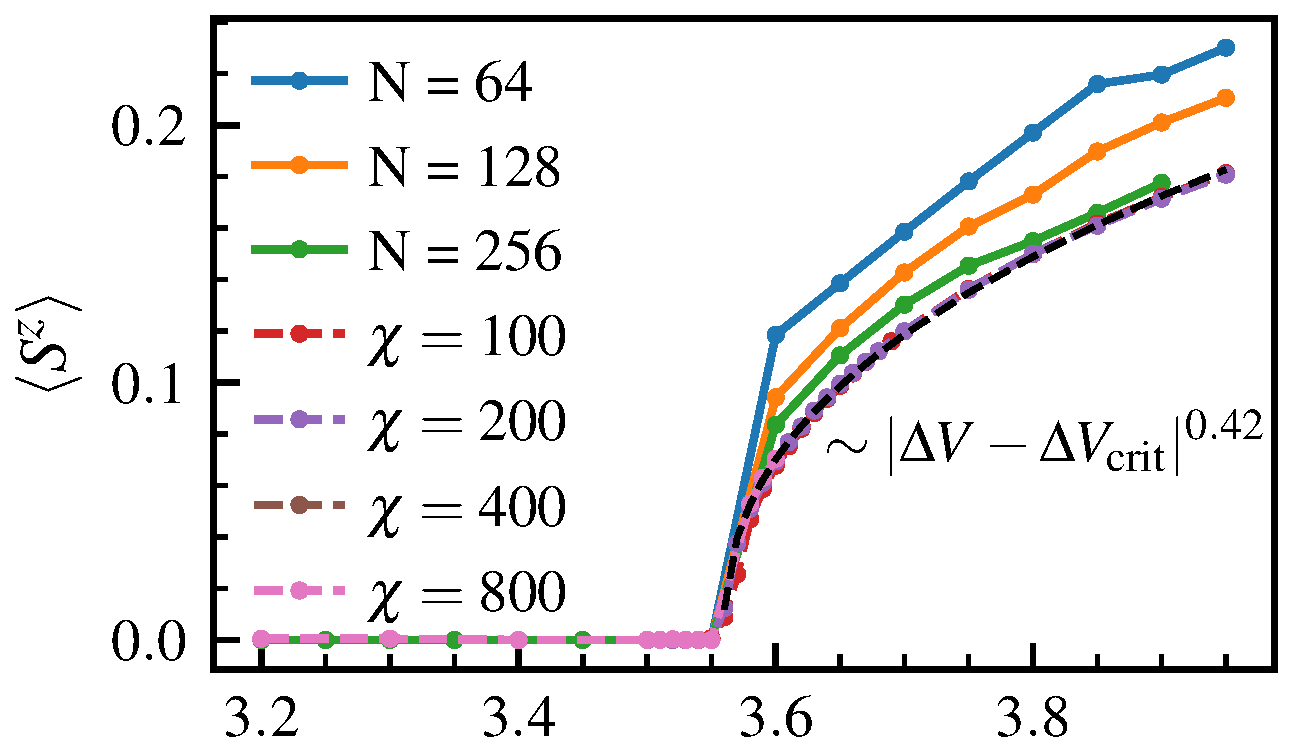
\includegraphics[width=\linewidth]{figures/paper_figS6_magnetization.png}\par
\vspace{0.05cm}
{\footnotesize $\langle S^z\rangle$ switches on \colorbox{cQCP!15}{\mystrut continuously} at $\Delta V_c$\par}
{\scriptsize DMRG, finite ($N$) and infinite ($\chi$) chains\par}}
\end{column}
\end{columns}
\onslide<3->{\tk{A continuous ferromagnetic transition: the critical point we study}}
\end{frame}
% Notes: Symmetry: the interactions depend only on S^z, so we have rotations of all spins about z (U(1): the theta of slide 1 is the spin angle in the xy plane) and the flip up<->down (Z2).
% Notes: Step 1: small Delta V: as many up as down spins, no magnetization: a Luttinger liquid in both charge and spin.
% Notes: Step 2: large Delta V: the spins polarize along z: an Ising-like ferromagnet, breaks the Z2.
% Notes: Step 3: DMRG: <S^z> switches on continuously at Delta V_c: a second-order transition, a quantum critical point. The FM side phase-separates (Nahum). The question of the talk: what does the U(1) do exactly at this point?
